% Beyond the Rate: Oral Presentation
% Academic Conference — Beamer
\documentclass[aspectratio=169, 11pt]{beamer}

% ── Theme ──
\usetheme{Madrid}
\usecolortheme{whale}
\usefonttheme{professionalfonts}
\setbeamertemplate{navigation symbols}{}
\setbeamertemplate{footline}{%
  \leavevmode\hbox{%
    \begin{beamercolorbox}[wd=.33\paperwidth,ht=2.5ex,dp=1ex,center]{author in head/foot}%
      \usebeamerfont{author in head/foot}\insertshortauthor
    \end{beamercolorbox}%
    \begin{beamercolorbox}[wd=.34\paperwidth,ht=2.5ex,dp=1ex,center]{title in head/foot}%
      \usebeamerfont{title in head/foot}\insertshorttitle
    \end{beamercolorbox}%
    \begin{beamercolorbox}[wd=.33\paperwidth,ht=2.5ex,dp=1ex,right]{date in head/foot}%
      \usebeamerfont{date in head/foot}\insertframenumber{}/\inserttotalframenumber\hspace*{2ex}
    \end{beamercolorbox}}%
  \vskip0pt%
}

% ── Packages ──
\usepackage{amsmath,amssymb}
\usepackage{graphicx}
\usepackage{booktabs}
\usepackage{tikz}
\usetikzlibrary{arrows.meta, positioning, calc}
\usepackage{hyperref}
\usepackage{appendixnumberbeamer}

% ── Colors ──
\definecolor{accent}{RGB}{43, 94, 167}
\definecolor{alertc}{RGB}{192, 57, 43}
\definecolor{success}{RGB}{39, 174, 96}

% ── Meta ──
\title[Beyond the Rate]{Beyond the Rate:\\Information Content of FOMC Forward Guidance Language}
\author[Yu \& Zhang]{Dechang Yu\inst{1} \and Eileen Zhang\inst{2}}
\institute[XJTLU]{\inst{1} Academy of AI, Xi'an Jiaotong-Liverpool University \and \inst{2} [Affiliation TBC]}
\date{Academic Conference 2026}

\begin{document}

% ═══════════════════════════════════════════════════════════════
% TITLE
% ═══════════════════════════════════════════════════════════════
\begin{frame}[plain]
\titlepage
\end{frame}

% ═══════════════════════════════════════════════════════════════
% OUTLINE
% ═══════════════════════════════════════════════════════════════
\begin{frame}{Outline}
\tableofcontents
\end{frame}

% ═══════════════════════════════════════════════════════════════
\section{Motivation}
% ═══════════════════════════════════════════════════════════════

\begin{frame}{The Puzzle}
\begin{columns}[T]
\column{0.55\textwidth}
\textbf{Central question:}\\
Does FOMC statement language convey information \alert{beyond} the rate decision?

\vspace{1em}
\textbf{Why it matters:}
\begin{itemize}
  \item Central banks increasingly rely on \textbf{forward guidance} as a policy tool
  \item Markets respond to \emph{what the Fed says}, not just \emph{what it does}
  \item The ``information channel'' (Romer \& Romer, 2000) suggests FOMC statements reveal the Fed's superior economic assessment
\end{itemize}

\column{0.42\textwidth}
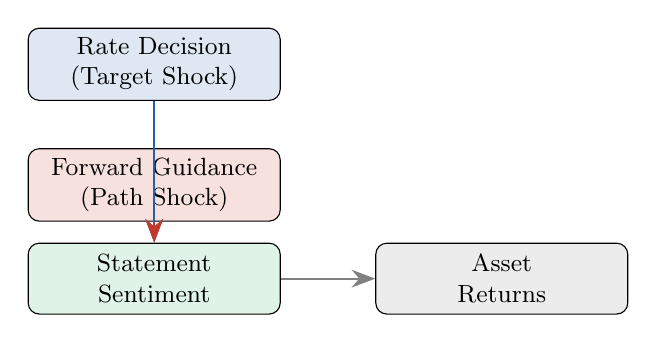
\begin{tikzpicture}[
  box/.style={draw, rounded corners, minimum width=3.2cm, minimum height=0.9cm, align=center, font=\small},
  arr/.style={-{Stealth[length=3mm]}, thick}
]
\node[box, fill=accent!15] (rate) {Rate Decision\\(Target Shock)};
\node[box, fill=alertc!15, below=0.6cm of rate] (fg) {Forward Guidance\\(Path Shock)};
\node[box, fill=success!15, below=1.8cm of rate] (sent) {Statement\\Sentiment};
\node[box, fill=gray!15, right=1.2cm of sent] (asset) {Asset\\Returns};
\draw[arr, accent] (rate) -- (sent);
\draw[arr, alertc] (fg) -- (sent);
\draw[arr, gray] (sent) -- (asset);
\end{tikzpicture}
\end{columns}
\end{frame}

% ═══════════════════════════════════════════════════════════════
\section{Literature \& Contribution}
% ═══════════════════════════════════════════════════════════════

\begin{frame}{Literature}
\begin{itemize}
  \item \textbf{Kuttner (2001)}: 30-min FF futures window $\rightarrow$ isolate monetary policy surprises
  \item \textbf{GSS (2005a)}: Decompose surprises into \textcolor{accent}{target} + \textcolor{alertc}{path} factors
  \item \textbf{Nakamura \& Steinsson (2018)}: High-frequency identification of monetary non-neutrality
  \item \textbf{Campbell et al.\ (2012)}: Delphic vs.\ Odyssean forward guidance
  \item \textbf{Jaroci\'{n}ski \& Karadi (2020)}: Separate policy shock from information shock
  \item \textbf{Hansen et al.\ (2018)}: Computational linguistics for FOMC transparency
\end{itemize}

\vspace{0.8em}
\textbf{Our contribution:}
\begin{enumerate}
  \item First to directly link \textbf{GSS target/path shocks} to \textbf{FOMC statement sentiment}
  \item Expanded CB dictionary (97 hawkish + 106 dovish terms, fully disjoint)
  \item Formal test of the \textbf{information channel} via text analysis
\end{enumerate}
\end{frame}

% ═══════════════════════════════════════════════════════════════
\section{Data \& Methodology}
% ═══════════════════════════════════════════════════════════════

\begin{frame}{Data}
\begin{columns}[T]
\column{0.48\textwidth}
\textbf{Monetary Policy Shocks}
\begin{itemize}
  \item Acosta (2022): 220 FOMC meetings, 1995--2022
  \item \textcolor{accent}{Target shock}: surprise in current FF rate
  \item \textcolor{alertc}{Path shock}: surprise in future rate path
  \item Extension: USMPD (SF Fed) $\rightarrow$ 2026
\end{itemize}

\vspace{0.5em}
\textbf{Market Data}
\begin{itemize}
  \item CRSP VW/EW/S\&P 500 via WRDS
  \item 117 meetings with complete overlap
\end{itemize}

\column{0.48\textwidth}
\textbf{FOMC Statement Sentiment}
\begin{itemize}
  \item 164 statements, 2006--2025
  \item Expanded CB dictionary:
    \begin{itemize}
      \item 97 hawkish terms
      \item 106 dovish terms
      \item 50 bigram phrases
      \item Fully disjoint
    \end{itemize}
  \item Score $= \frac{H - D}{H + D + \epsilon}$
  \item Validated: $r = 0.29$ with rate change
\end{itemize}
\end{columns}
\end{frame}

\begin{frame}{Empirical Strategy}
\textbf{Four hypotheses:}

\vspace{0.5em}
\begin{tabular}{lll}
\toprule
Hypothesis & Prediction & Specification \\
\midrule
H1 & Shocks predict sentiment & $S_t = \alpha + \beta_1 \text{Target}_t + \beta_2 \text{Path}_t + \varepsilon_t$ \\
H2 & Shocks predict returns & $R_t = \alpha + \beta_1 \text{Target}_t + \beta_2 \text{Path}_t + \varepsilon_t$ \\
H3 & Path $>$ Target for sentiment & $|\beta_2| > |\beta_1|$ in H1 \\
H4 & Stronger during FG period & Interaction with FG dummy \\
\bottomrule
\end{tabular}

\vspace{0.8em}
\textbf{Estimation:} OLS with Newey-West (lag=1) standard errors

\vspace{0.3em}
\textbf{Sample:} 117 FOMC meetings, January 2006 -- July 2022
\end{frame}

% ═══════════════════════════════════════════════════════════════
\section{Main Results}
% ═══════════════════════════════════════════════════════════════

\begin{frame}{H1: Sentiment and Monetary Policy Shocks}
\begin{columns}[T]
\column{0.55\textwidth}
\begin{tabular}{lcc}
\toprule
 & Coefficient & $p$-value \\
\midrule
Target shock & 0.000290 & 0.062\textsuperscript{*} \\
Path shock & 0.000469 & 0.047\textsuperscript{**} \\
\midrule
$R^2$ & \multicolumn{2}{c}{4.06\%} \\
$N$ & \multicolumn{2}{c}{117} \\
\bottomrule
\end{tabular}

\vspace{0.5em}
\small
\textsuperscript{***}$p<0.01$, \textsuperscript{**}$p<0.05$, \textsuperscript{*}$p<0.10$

\vspace{0.5em}
\textbf{Key finding:} Path shock is significant at 5\%, target at 10\%.\\
\alert{But:} Wald test $\chi^2 = 0.19$, $p = 0.66$ --- cannot reject $\beta_1 = \beta_2$.

\column{0.42\textwidth}
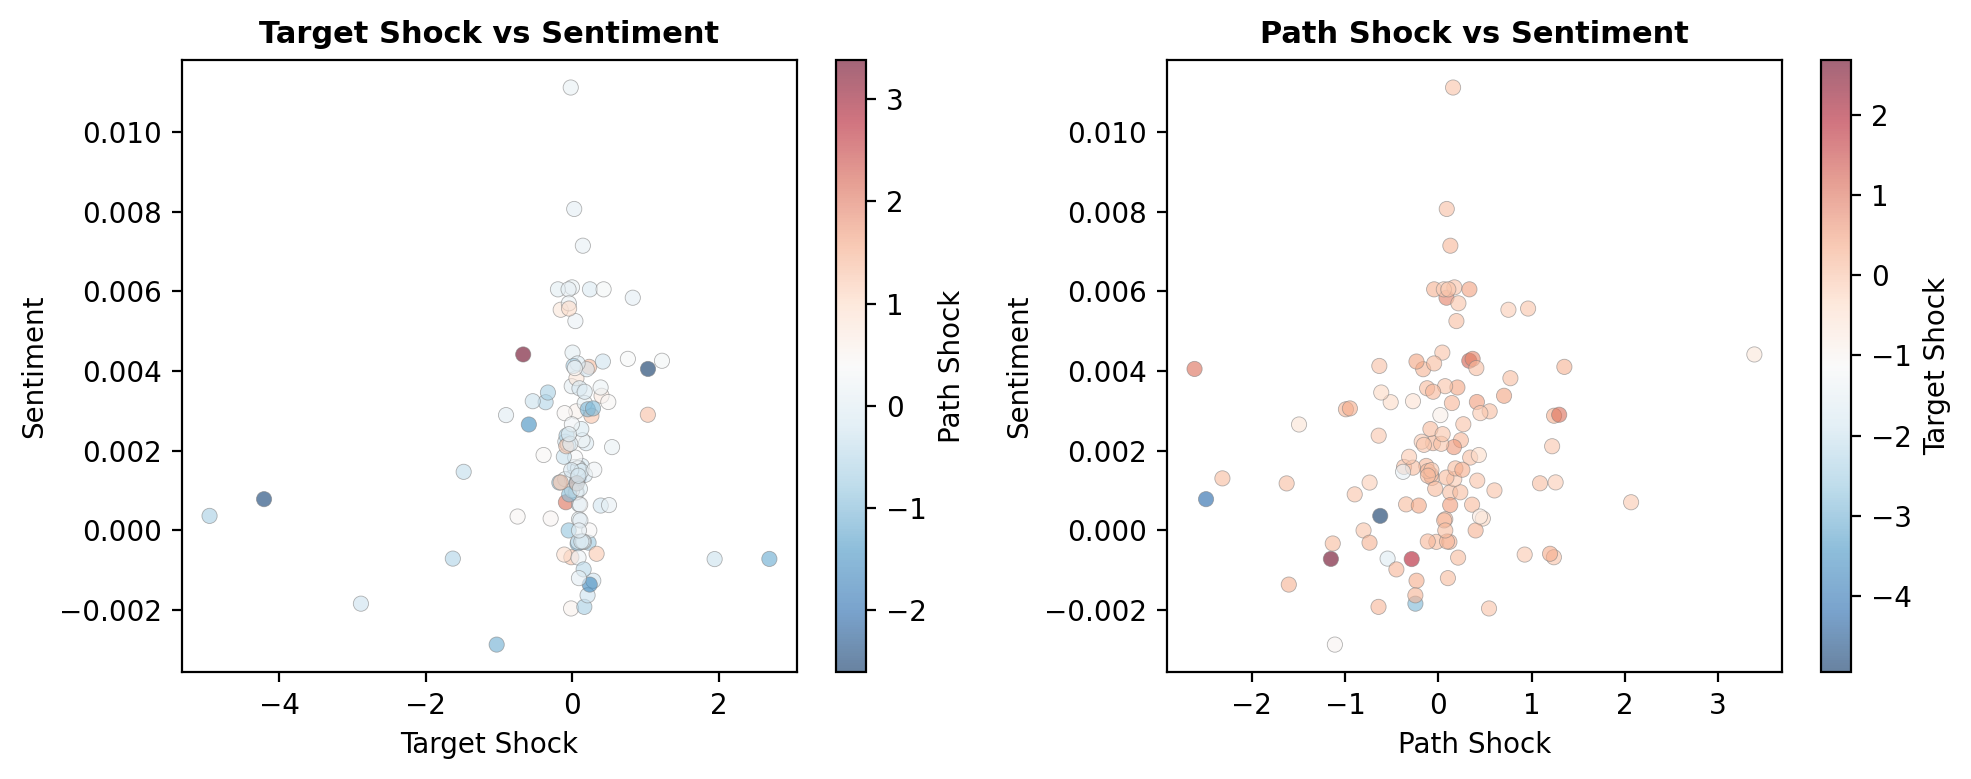
\includegraphics[width=\textwidth]{figures/fig2_scatter.png}
\end{columns}
\end{frame}

\begin{frame}{H2: Asset Returns and Shocks}
\begin{columns}[T]
\column{0.55\textwidth}
\begin{tabular}{lcccc}
\toprule
Asset & $\beta_T$ & $p_T$ & $\beta_P$ & $p_P$ \\
\midrule
CRSP VW & $-0.435$ & 0.111 & $-0.186$ & 0.398 \\
CRSP EW & $-0.449$ & 0.044\textsuperscript{**} & $-0.174$ & 0.421 \\
S\&P 500 & $-0.391$ & 0.158 & $-0.179$ & 0.395 \\
\midrule
\multicolumn{5}{l}{Returns in percentage points; $N = 117$} \\
\bottomrule
\end{tabular}

\vspace{0.5em}
\textbf{Findings:}
\begin{itemize}
  \item Target shock: significant for EW (small-cap), not VW
  \item Path shock: \alert{not significant} for any asset
  \item Small-cap sensitivity consistent with literature
\end{itemize}

\column{0.42\textwidth}
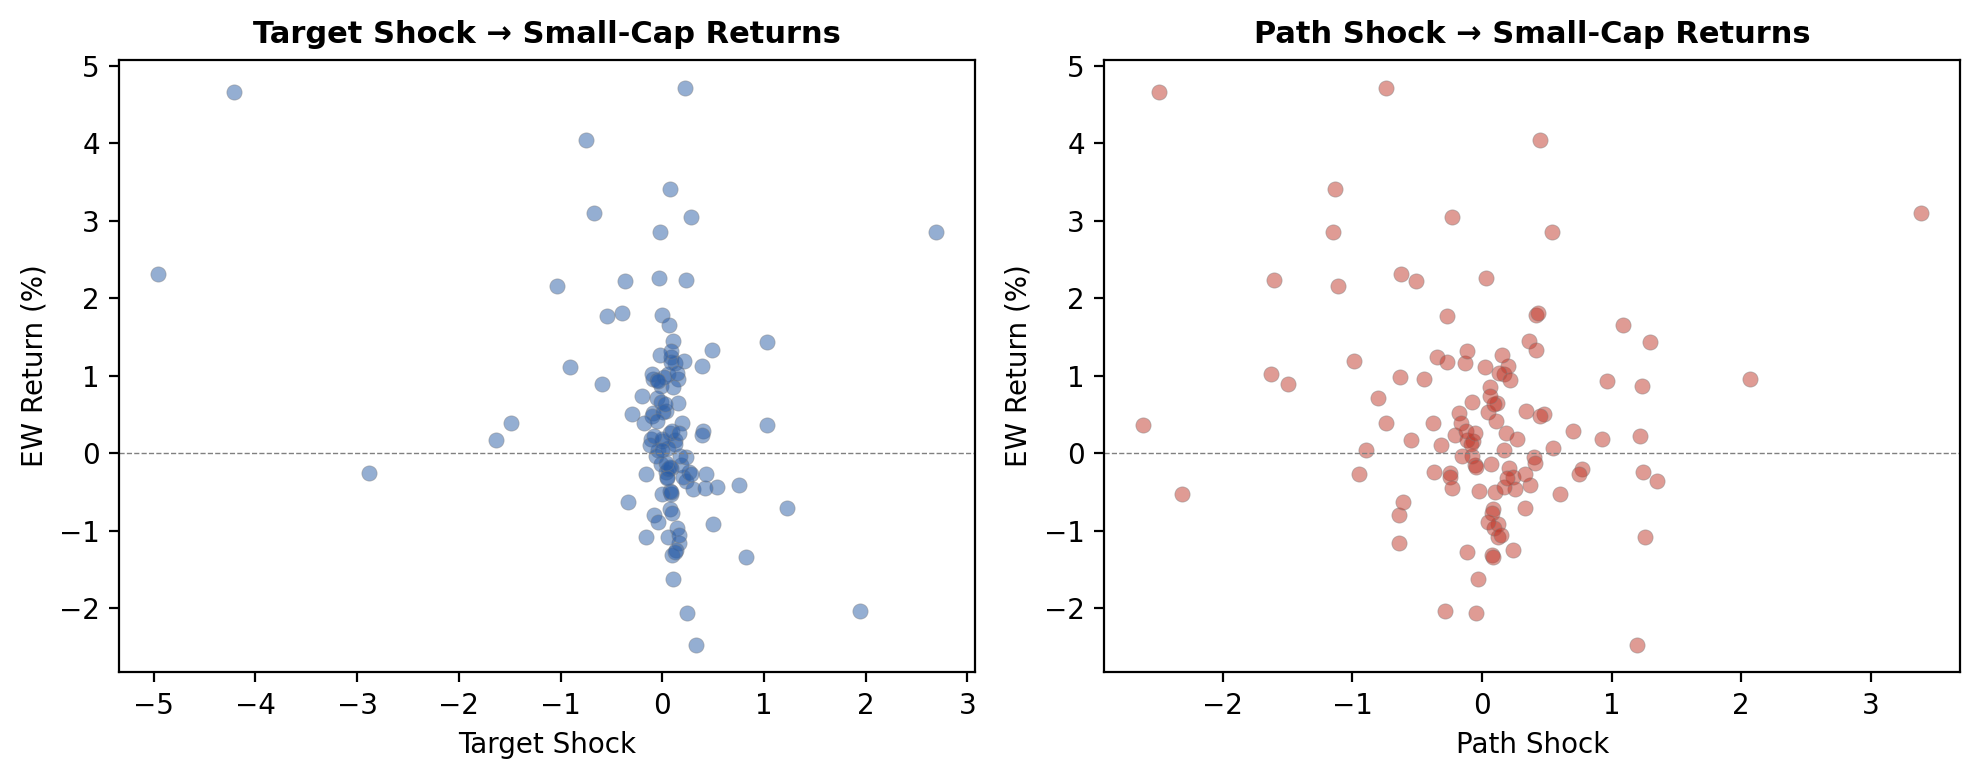
\includegraphics[width=\textwidth]{figures/fig3_h2.png}
\end{columns}
\end{frame}

\begin{frame}{H3: The Information Channel}
\textbf{Prediction:} Path shock has larger effect on sentiment than target shock.

\vspace{0.5em}
\begin{itemize}
  \item $|t_{\text{path}}| = 2.012 > |t_{\text{target}}| = 1.887$
  \item Path significant at 5\%, target at 10\%
  \item \alert{But:} Wald test $H_0\!: \beta_{\text{target}} = \beta_{\text{path}}$
    \begin{itemize}
      \item $\chi^2 = 0.19$, $p = 0.66$
      \item Cannot reject equality
    \end{itemize}
\end{itemize}

\vspace{0.5em}
\textbf{Interpretation:} \textit{Suggestive} evidence consistent with the information channel, but \textbf{not definitive proof} that the path effect dominates.

\vspace{0.5em}
\textbf{Why the modest $R^2$ (4.06\%):}
\begin{itemize}
  \item 96\% of sentiment variation is unexplained by shocks
  \item Likely reflects: economic data releases, institutional inertia, other Fed communication channels
\end{itemize}
\end{frame}

% ═══════════════════════════════════════════════════════════════
\section{Robustness}
% ═══════════════════════════════════════════════════════════════

\begin{frame}{Robustness Checks}
\begin{tabular}{lccccc}
\toprule
Sample & $R^2$ & $p$(Target) & $p$(Path) & $N$ & Period \\
\midrule
Full (Acosta) & 4.06\% & 0.062\textsuperscript{*} & 0.047\textsuperscript{**} & 117 & 2006--22 \\
No COVID & 4.10\% & 0.075\textsuperscript{*} & 0.042\textsuperscript{**} & 115 & 2006--22 \\
Post-2010 & 2.02\% & 0.369 & 0.108 & 97 & 2010--22 \\
Extended & 1.65\% & 0.419 & 0.058\textsuperscript{*} & 163 & 2006--26 \\
\bottomrule
\end{tabular}

\vspace{0.8em}
\textbf{Key takeaways:}
\begin{itemize}
  \item COVID exclusion: virtually unchanged $\rightarrow$ not driven by outliers
  \item Post-2010: neither shock significant $\rightarrow$ ZLB period weakens the signal
  \item Extended sample (USMPD): path still significant at 10\% through 2026
\end{itemize}
\end{frame}

\begin{frame}{Regime-Specific Results}
\begin{tabular}{lcccc}
\toprule
Period & $N$ & $R^2$ & $p$(Target) & $p$(Path) \\
\midrule
Pre-ZLB (2006--08) & 8 & 20.5\% & 0.360 & 0.403 \\
Crisis (2008--10) & 12 & 9.2\% & 0.930 & 0.124 \\
ZLB/FG (2010--16) & 48 & 7.5\% & 0.249 & 0.107 \\
Normalization (2016--20) & 30 & 13.3\% & 0.009\textsuperscript{***} & 0.873 \\
COVID+ (2020--22) & 19 & 3.6\% & 0.355 & 0.953 \\
\bottomrule
\end{tabular}

\vspace{0.5em}
\small\textit{Caution: small $N$ within each regime. Results are suggestive.}

\vspace{0.3em}
\textbf{Pattern:} Target dominates during Normalization (rate hikes); Path is more relevant during ZLB/FG and Crisis periods.
\end{frame}

% ═══════════════════════════════════════════════════════════════
\section{Discussion}
% ═══════════════════════════════════════════════════════════════

\begin{frame}{Limitations \& Future Work}
\textbf{Limitations:}
\begin{enumerate}
  \item \textbf{Low $R^2$}: Shocks explain only 4\% of sentiment variation
  \item \textbf{No control variables}: No lagged sentiment, macro controls, or meeting type dummies
  \item \textbf{Dictionary-based sentiment}: Cannot capture context or pragmatics
  \item \textbf{Sample size}: $N = 117$ limits power, especially for sub-sample analysis
  \item \textbf{US only}: External validity to other central banks unknown
  \item \textbf{Multiple testing}: 4 hypotheses without significance level adjustment
\end{enumerate}

\vspace{0.5em}
\textbf{Future directions:}
\begin{itemize}
  \item FinBERT / LLM-based sentiment for better measurement
  \item Control variables: lagged sentiment, macro indicators
  \item Cross-country: ECB, BoJ, BoE
  \item Other channels: minutes, press conferences, speeches
\end{itemize}
\end{frame}

% ═══════════════════════════════════════════════════════════════
\section{Conclusion}
% ═══════════════════════════════════════════════════════════════

\begin{frame}{Conclusion}
\begin{enumerate}
  \item The \textbf{path shock} (forward guidance) is a statistically significant predictor of FOMC statement sentiment ($p = 0.047$)
  \item The \textbf{target shock} is also significant at 10\% ($p = 0.062$)
  \item However, we \textbf{cannot formally establish} that the path effect dominates (Wald test $p = 0.66$)
  \item The evidence is \textbf{suggestive} of an information channel, not definitive
  \item Asset returns respond primarily to the \textbf{target shock} (small-cap sensitivity), not the path shock
  \item Results are robust to COVID exclusion and sample extension (USMPD through 2026)
\end{enumerate}

\vspace{0.5em}
\centering
\textbf{Takeaway:} FOMC language is forward-looking, but monetary policy shocks explain only a small fraction of its variation. The information channel exists but is one of many forces shaping central bank communication.
\end{frame}

\begin{frame}[plain]
\centering
\vspace{2cm}
{\Huge\bfseries Thank You}\\[1.5em]
{\Large Questions \& Discussion}\\[2em]
{\normalsize Dechang Yu \quad|\quad dechang64@github}\\[0.5em]
{\small Academy of AI, Xi'an Jiaotong-Liverpool University}
\end{frame}

% ═══════════════════════════════════════════════════════════════
\appendix
% ═══════════════════════════════════════════════════════════════

\begin{frame}{Appendix: USMPD Factor Replication}
\textbf{GSS (2005a) two-step orthogonalized PCA:}
\begin{enumerate}
  \item Target = 1st PC of [MP1, FF1--FF4]
  \item Path = 1st PC of [FF4--FF6, ED2--ED4], orthogonalized against target
  \item Normalized by regressing on daily 1Y GSW yield change
\end{enumerate}

\vspace{0.5em}
\begin{tabular}{lccc}
\toprule
Factor & Instruments & PC1 Variance & Corr w/ Acosta \\
\midrule
Target & MP1, FF1--FF4 & 87.1\% & 0.958 \\
Path (orth) & FF4--FF6, ED2--ED4 & 77.0\% & 0.970 \\
STMT (single) & MP1, MP2, ED2--ED4 & 78.5\% & 0.989 (target+path) \\
\bottomrule
\end{tabular}

\vspace{0.5em}
Single-factor STMT replicates perfectly ($r = 1.000$).
\end{frame}

\end{document}
